\documentclass[tikz,border=5pt]{standalone}
\usepackage{luatexja}
\usepackage[hiragino-pron]{luatexja-preset}
\usepackage{amsmath,amssymb}
\usepackage{pgfplots}
\pgfplotsset{compat=1.18}
\usetikzlibrary{arrows.meta,patterns}

\begin{document}
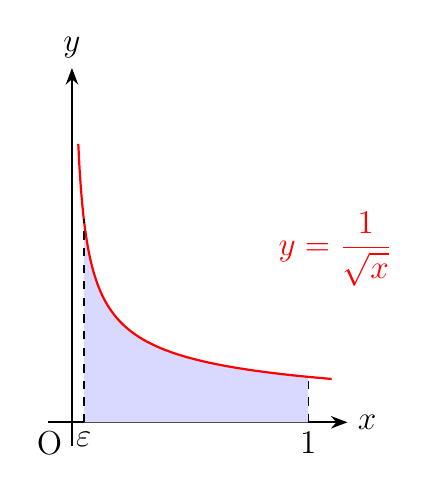
\begin{tikzpicture}[every node/.style={font=\large}]
  % Axes
  \draw[-{Stealth[length=6pt]}, thick] (-0.3,0) -- (3.5,0) node[right] {$x$};
  \draw[-{Stealth[length=6pt]}, thick] (0,-0.3) -- (0,4.5) node[above] {$y$};

  % Shaded region
  \fill[blue!15, domain=0.15:3, samples=100]
    (0.15,0) -- plot (\x, {1/sqrt(\x)}) -- (3,0) -- cycle;

  % Curve y = 1/sqrt(x)
  \draw[thick, red, domain=0.08:3.3, samples=200] plot (\x, {1/sqrt(\x)});

  % Epsilon line
  \draw[dashed, thick] (0.15,0) -- (0.15,{1/sqrt(0.15)});

  % Labels
  \node[below] at (0.15,0) {$\varepsilon$};
  \node[below] at (3,0) {$1$};
  \draw[dashed] (3,0) -- (3,{1/sqrt(3)});
  \node[right, red] at (2.5,2.2) {$y = \dfrac{1}{\sqrt{x}}$};

  % Origin
  \node[below left] at (0,0) {O};
\end{tikzpicture}
\end{document}
